% Chapter 3
\chapter{Thu thập dữ liệu} % Main chapter title
\label{Chapter3}

\section{Các nguồn chia sẻ dữ liệu} % Main chapter title
\subsection{HERE Real-time Traffic}
HERE Real-time Traffic là một dịch vụ của HERE Technologies - một công ty nổi tiếng và có kinh nghiệm trong việc cung cấp các dịch vụ về bản đồ và vị trí. Dịch vụ trên giúp người dùng có thể xác định vị trí, thời gian và lý do tắc nghẽn giao thông xảy ra bằng cách cung cấp tình trạng giao thông và các sự cố từng phút. Nguồn dữ liệu của dịch vụ được cung cấp và phân tích từ nhiều nguồn tổng hợp như cảm biến của ôtô, các cảm biến cố định trên đường hoặc từ các thiết bị sử dụng các ứng dụng của công ty. Năm 2017, HERE thông báo dịch vụ HERE Real-time Traffic cũng đã hỗ trợ ở Việt Nam.\cite{HERE}

\begin{figure}[!ht]
	\begin{center}
		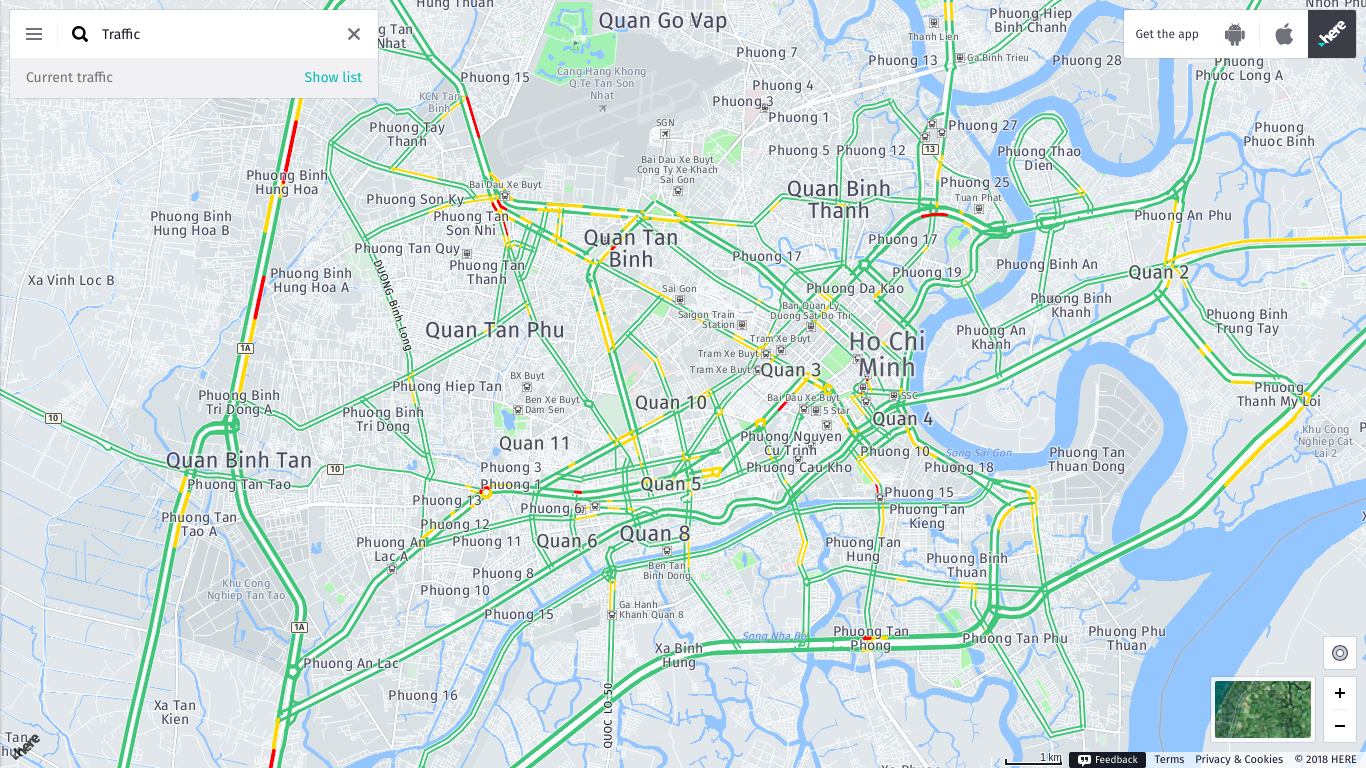
\includegraphics[width=1.0\textwidth]{images/here_maps.png}
	\end{center}
	\caption{HERE Real-time Traffic được sử dụng trên Here maps}
\end{figure}

HERE giới thiệu rằng dịch vụ cung cấp nguồn dữ liệu thời gian thực và có độ chính xác cao. Tuy nhiên, lượng người sử dụng dịch vụ này ở Việt Nam còn thấp, do đó độ tin cậy của dữ liệu không cao. Nhóm quyết định tạm dừng việc sử dụng dữ liệu từ HERE để đảm bảo độ chính xác của hệ thống.
\subsection{Smart BK Traffic}
Hệ thống giao thông thông minh (Smart BK Traffic) là hệ thống được nhóm Intelligent Transportation Systems Group (ITSG) tại trường Đại học Bách Khoa phát triển. Hệ thống được xây dựng để thu thập xử lý tín hiệu GPS từ xe hơi, xe taxi, xe buýt, thiết bị di động; đồng thời cung cấp dữ liệu đã được xử lý đến các ứng ụng web và điện thoại thông minh theo thời gian thực.

\begin{figure}[!ht]
	\begin{center}
		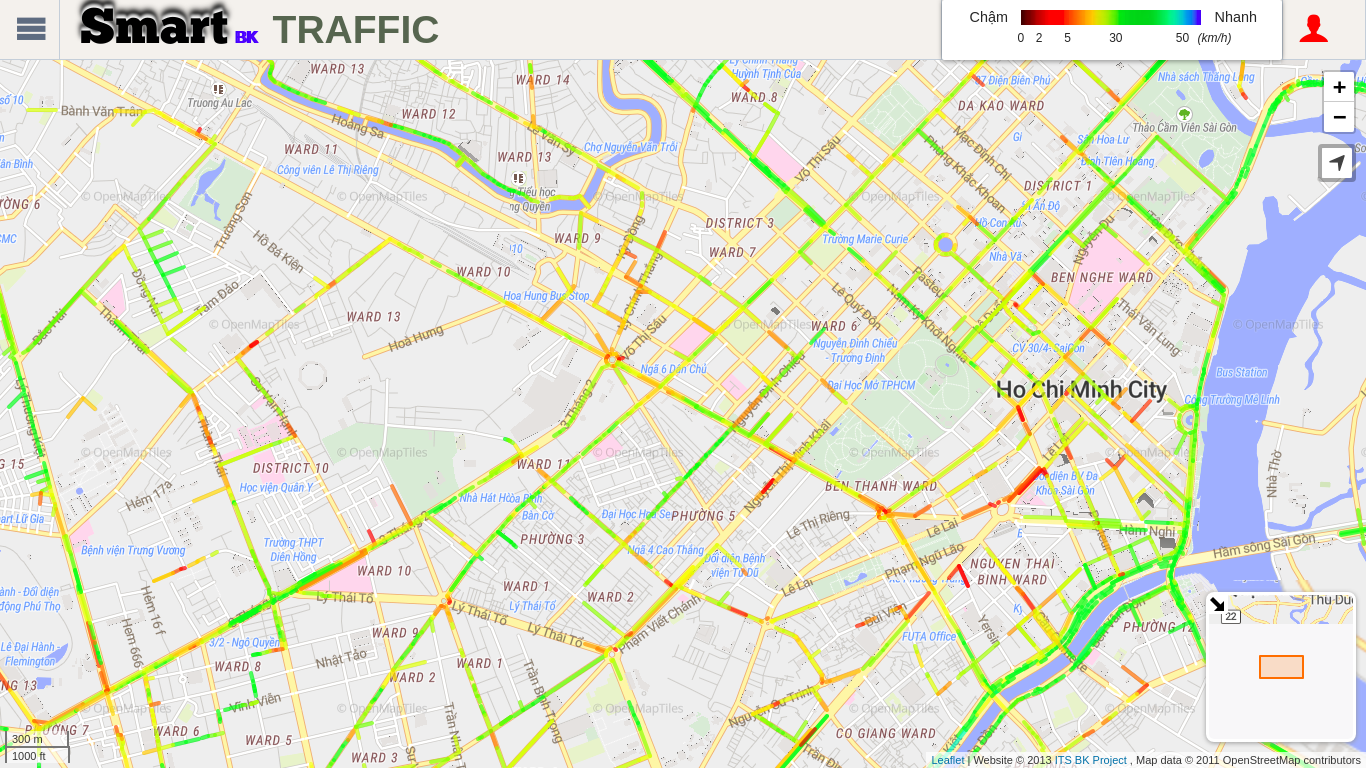
\includegraphics[width=1.0\textwidth]{images/smartbktraffic.png}
	\end{center}
	\caption{Website của hệ thống Smart BK Traffic - 17:45 08/12/2018}
\end{figure}

Sau một thời gian tìm hiểu và đánh giá, nhóm nhận thấy dữ liệu do hệ thống Smart BK Traffic cung cấp tương đối chính xác đối với tình trạng giao thông của thành phố Hồ Chí Minh. Mặc dù dữ liệu vẫn bị thiếu ở một số tuyến đường nhưng nhìn chung vẫn khá đầy đủ. Do đó, nhóm quyết định sử dụng nguồn dữ liệu này, kết hợp với nguồn dữ liệu crowdsourcing để có thể khai phá, đưa ra dự đoán tình hình giao thông ở những đoạn đường bị thiếu nhằm bổ sung vào những thiếu sót mà hệ thống đang có. Chi tiết về cách thu thập cũng như sử dụng dữ liệu sẽ được nhóm trình bày vào phần 3.2

\subsection{Dữ liệu từ cộng đồng (Crowdsourcing)}
Như đã trình bày ở trên, nguồn dữ liệu thu thập được từ cộng đồng là một nguồn dữ liệu quan trọng và không thể thiếu trong quá trình làm đề tài. Một ví dụ cho tính hiệu quả của việc sử dụng nguồn dữ liệu cộng đồng ở Việt Nam là hệ thống VOV Giao thông 91Mhz của Đài tiếng nói Việt Nam, với cách thức thông báo tình trạng giao thông thông qua sóng radio với nguồn thông tin chính xác đến từ các tài xế lái xe, từ đó giúp cho các tài xế khác có thể điều chỉnh lộ trình của mình cho phù hợp, tránh đi những tuyến đường bị kẹt xe. Tuy nhiên việc sử dụng dữ liệu cộng đồng như thế vẫn còn rất nhiều hạn chế, cho nên cần một giải pháp khác để khai thác, sử dụng hiệu quả nguồn dữ liệu từ cộng đồng hơn. Một vài nhóm nghiên cứu nước ngoài cũng đã thực hiện một số công trình nghiên cứu về việc áp dụng kỹ thuật thu thập dữ liệu cộng đồng (crowdsourcing) để giải quyết các bài toán thu thập dữ liệu nói chung, và giao thông nói riêng \cite{CROWND1} \cite{CROWND2} \cite{CROWND3} \cite{CROWND4}. Từ những nghiên cứu nói trên, nhóm kết hợp với hai nhóm khác cũng làm đề tài liên quan đến giao thông để xây dựng hệ thống cung cấp thông tin giao thông theo thời gian thực cho người dùng thông qua ứng dụng di động, với nguồn dữ liệu đến từ chính cộng đồng người dùng của ứng dụng.

\section{Kỹ thuật thu thập dữ liệu}
\subsection{Smart BK Traffic}
Sau quá trình tìm hiểu ngắn, nhóm nhận thấy hệ thống Smart BK Traffic cung cấp một số API để có thể lấy được dữ liệu về tình trạng giao thông thành phố Hồ Chí Minh tại thời điểm sử dụng. Trong đó, API quan trọng nhất được nhóm sử dụng là:
\begin{itemize}
    \item \textit{https://traffic.hcmut.edu.vn/hcm/rest/tc/init?} với các tham số truyền vào là tọa độ của 4 góc bản đồ cần lấy dữ liệu và độ zoom của map, cụ thể là:
\begin{itemize}
    \item latTL, lonTL: vĩ độ, kinh độ của điểm góc trên cùng bên trái
    \item latTR, lonTR: vĩ độ, kinh độ của điểm góc trên cùng bên phải
    \item latBL, lonBL: vĩ độ, kinh độ của điểm góc dưới cùng bên trái
    \item latBR, lonBR: vĩ độ, kinh độ của điểm góc dưới cùng bên phải
    \item zoom: độ zoom của bản đồ
\end{itemize}
    API trên trả về dữ liệu giao thông ở thời điểm gọi API và có cấu trúc như sau:
\begin{lstlisting}[language=XML]
{
  "segs": [
    {
      "v": "lat1,lon1,lat2,lon2,velocity,description,accuracy,id"
    }
  ],
  "last": boolean,
  "key": "key"
}
\end{lstlisting}
    Trong đó:
    \begin{itemize}
        \item "segs": là một mảng các segment, thông tin mỗi segment được lưu trong field "v" với các thuộc tính được phân cách nhau bằng dấu phẩy:
        \begin{itemize}
            \item lat1,lon1: vĩ độ, kinh độ điểm đầu của segment
            \item lat2,lon2: vĩ độ, kinh độ điểm cuối của segment
            \item velocity: vận tốc trên đoạn segment đó 
            \item description: miêu tả về đoạn segment
            \item accuracy: độ chính xác của giá trị vận tốc
            \item id: id của field "v".
        \end{itemize}
    
    \item "last": có giá trị boolean để xác định segment trả về đã là cuối cùng hay chưa. Nếu chưa thì sẽ có giá trị bằng \textit{false} và tạo ra key ở field "key" để có thể tiếp tục get dữ liệu.
    \item "key": tham số của API \textit{https://traffic.hcmut.edu.vn/hcm/rest/?key=} để get tiếp dữ liệu các segment còn thiếu.
    \end{itemize}
\end{itemize}
Sau khi đã hiểu rõ được cách làm việc của API, nhóm viết một chương trình nhỏ chạy trên server để lấy dữ liệu toàn thành phố Hồ Chí Minh mỗi 15 phút và lưu xuống database Mongodb.

Để lấy được dữ liệu của toàn thành phố, nhóm xác định bốn điểm tọa độ của vùng bao phủ thành phố và từ đó chia nhỏ ra thành 16x16 vùng nhỏ hơn để có thể thu thập dữ liệu được chính xác hơn. Vì nếu chỉ sử dụng bốn điểm tọa độ của vùng bao phủ thành phố thì API chỉ trả về dữ liệu của một số tuyến đường quan trọng trên bản đồ, dẫn đến sự thiếu sót dữ liệu. Sau khi xác định được các vùng nhỏ để tránh sự thiếu sót dữ liệu, nhóm sử dụng các API trình bày ở trên để thu thập và lưu dữ liệu theo cấu trúc của các model mà nhóm đã thảo luận, thống nhất với hai nhóm làm đề tài giao thông khác. Chi tiết về thiết kế cơ sở dữ liệu sẽ được trình bày ở phần 5.

\subsection{Dữ liệu từ cộng đồng (Crowdsourcing)}
Ở giai đoạn đề cương luận văn, việc thu thập dữ liệu từ cộng đồng chỉ dừng lại ở những bước xây dựng nền tảng để có thể thực hiện thu thập dữ liệu ở giai đoạn sau. Do đó, nhóm tham gia thảo luận với hai nhóm làm đề tài giao thông còn lại và đưa ra các đánh giá, nhận xét để xây dựng mô hình quan hệ thực thể, cấu trúc dữ liệu, thảo luận các phương pháp đánh giá tính xác thực của dữ liệu. Về việc xây dựng ứng dụng di động để thu thập dữ liệu từ cộng đồng, nhóm chỉ tham gia hỗ trợ chứ không trực tiếp xây dựng nên ở phạm vi đề cương luận văn này, nhóm chỉ trình bày sơ lược cách thu thập dữ liệu từ cộng đồng thông qua ứng dụng.

Cụ thể, sau khi người dùng cài đặt ứng dụng, người dùng có thể gửi những báo cáo liên quan đến tình trạng giao thông ở đoạn đường xảy ra kẹt xe. Báo cáo sẽ bao gồm các thông tin như thông tin đoạn đường, vận tốc hiện tại của đoạn đường, thời gian, mô tả, hình ảnh. Dữ liệu báo cáo sẽ được gửi lên server để lưu trữ cho việc phân tích, đồng thời gửi cảnh báo đến những người dùng khác về tình trạng giao thông ở đoạn đường đó. Từ đó, người dùng khác nếu ở gần sẽ có thể đánh giá độ chính xác của báo cáo đó. Để việc báo cáo được đơn giản hơn, ba nhóm cũng thảo luận, nghiên cứu đưa công nghệ speech to text áp dụng vào việc gửi báo cáo. Đồng thời, đưa ra các hình thức khuyến khích người dùng chia sẽ dữ liệu bằng hệ thống vinh danh, quà tặng.
